\documentclass{article}

\usepackage{graphicx}
\usepackage{subcaption}
\usepackage{amssymb}
\usepackage[utf8]{inputenc}
\usepackage[T1]{fontenc}

\renewcommand{\familydefault}{\sfdefault}
\usepackage[scaled=1]{helvet}
\usepackage[helvet]{sfmath}
\everymath={\sf}

\title{Reporte de Actividad 3}

\author{Diego Iván Moreno Campa}

\date{8 de Febrero, 2018}

\begin{document}

\maketitle

\bigskip

\section{Introducción}

Esta actividad es el tercer trabajo para la materia de Física computacional I en la licenciatura de Física.

El propósito de la actividad es practicar el análisis de datos sobre dos archivos creados por sondeos meteorológicos, uno en diciembre y otro en junio, para comparar las variaciones entre las estaciones. En esta actividad utilizaremos Pandas para organizar los datos obtenidos y matplotlib para gráficarlos, las cuales examinaremos para observar relaciones.

\section{Fundamentos}

Para comprender los datos que estamos graficando primeramente debemos conocer que es un sondeo atmosférico y que tipo de datos nos entregara para de esta forma interpretar lo que veremos.

El sondeo atmosférico es una medición de la distribución vertical de propiedades físicas de columnas atmosféricas como lo son la presión, temperatura, velocidad del viento y dirección, contenido de agua liquida, concentración de ozono, contaminación, entre otras propiedades. Tales mediciones se realizan con el flujo de la naturaleza, llamadas \textit{in situ} como lo son los sondeos por globos meteorológicos o a través de aviones, o son medidas a distancia, como lo son en estaciones terrestres utilizando microondas.
Con esto nos podemos familiarizar con los archivos de datos y entender que las mediciones realizadas por la universidad de Wyoming, de donde obtendremos los datos, se realizaron utilizando globos meteorológicos y por ende, cada medición se lleva a cabo mientras asciende el globo.

\section{Análisis de datos}

Primeramente necesitaremos dos muestras en forma de archivos de texto de datos por sondeo de globo metereológico tomadas de la página de la universidad de Wyoming, capturadas en los días 22 de diciembre de 2017 y 22 de junio de 2017. Para propósitos de esta práctica se tomaron los datos de la ciudad de Albuquerque, Nuevo México.

Comenzamos importando las librerías necesarias para esta actividad, las cuales son Pandas, NumPy y MatplotLib como en la práctica anterior. Ahora bien, para leer los archivos que no tienen la forma con la que se pueden leer utilizando Pandas por lo que se utilizó una función anónima para excluir la lectura de ciertos renglones con puro texto:
\begin{figure}[h!]
\centering
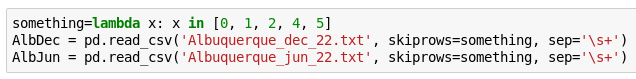
\includegraphics[width=300px,height=32px]{1stInst.png}
\end{figure}

Para asegurarse de que los datos hayan sido leídos correctamente, se imprime el encabezado de los datos ya estructurados dentro de Python:
\begin{figure}[h!]
\centering
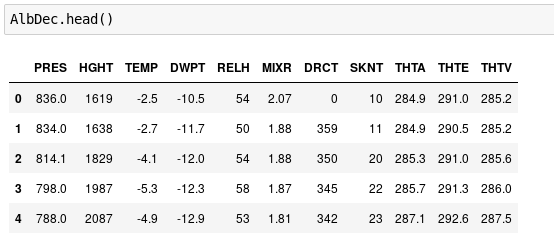
\includegraphics[width=277px,height=121px]{2ndInst.png}
\end{figure}
\begin{itemize}
\item \textbf{PRES}: columna de Presión medida en hectapascales
\item \textbf{HGHT}: columna de la altura medida en metros
\item \textbf{TEMP}: columna de la temperatura medida en grados Celsius
\item \textbf{DWPT}: columna de la temperatura de rocío medida en grados Celsius
\item \textbf{RELH}: columna de la humedad relativa medida en porcentaje \%
\item \textbf{MIXR}: columna de la Razón Mixta medida en gramos por kilogramo
\item \textbf{DRCT}: columna de la dirección del viento medida en grados
\item \textbf{SKNT}: columna de la velocidad de los vientos medida en nudos
\item \textbf{THTA, THTE Y THTV}: columnas de variables termodinámicas medidas en Kelvin
\end{itemize}

Enseguida se nos pidió graficar la presión en función de la altura, lo cual se realizó definiendo una variable que tomara únicamente los valores de las columnas de PRES y HGHT, después se utilizó el comando plot(x='HGHT') para especificar el eje coordenado.
\begin{figure}[h!]
	\begin{subfigure}[b]{0.5\linewidth}
    \raggedleft
	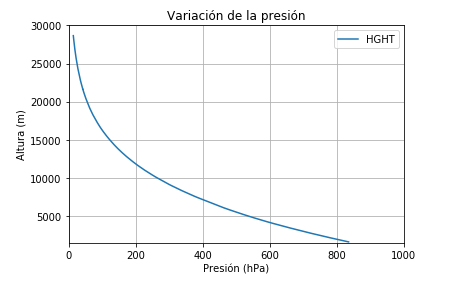
\includegraphics[width=\linewidth]{3rdInst.png}
    \caption{22/Dic/2017}
	\end{subfigure}
	\begin{subfigure}[b]{0.5\linewidth}
    \raggedright
	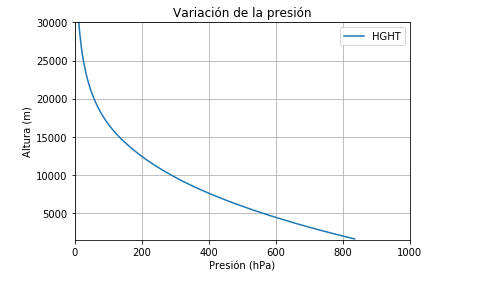
\includegraphics[width=\linewidth]{3rdInstJun.png}
	\caption{22/Jun/2017}
    \end{subfigure}
    \caption{Variación de la presión}
\end{figure}

Luego se nos pidió graficar la variación de la temperatura en función de la altura, lo cual se realizó de la misma manera que las gráficas anteriores.
\begin{figure}[h!]
	\begin{subfigure}[b]{0.5\linewidth}
    \raggedleft
	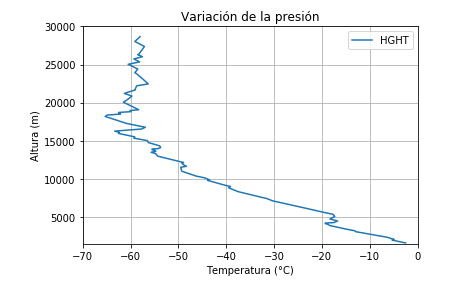
\includegraphics[width=\linewidth]{4thInstDec.png}
    \caption{22/Dic/2017}
	\end{subfigure}
	\begin{subfigure}[b]{0.5\linewidth}
    \raggedright
	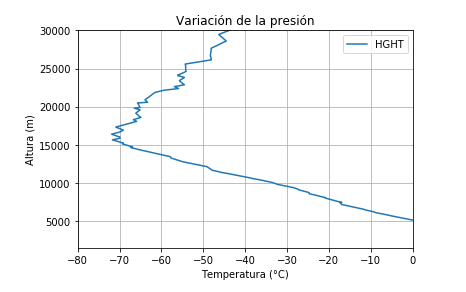
\includegraphics[width=\linewidth]{4thInstJun.png}
    \caption{22/Jun/2017}
	\end{subfigure}
    \caption{variación de la temperatura}
\end{figure}

Después se utilizaron las columnas de TEMP, DWPT y HGHT para gráficar la temperatura y la temperatura de rocío en función de la altura utilizando la misma secuencia de comandos que las gráficas anteriores con la excepción de que ahora la variable anteriormente creada para seleccionar únicamente dos columnas ahora toma tres.
\begin{figure}[ht!]
	\begin{subfigure}[b]{0.5\linewidth}
    \raggedleft
	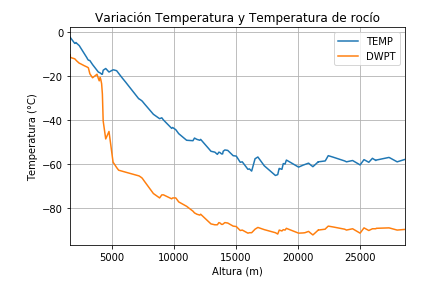
\includegraphics[width=\linewidth]{5thInstDec.png}
    \caption{22/Dic/2017}
	\end{subfigure}
	\begin{subfigure}[b]{0.5\linewidth}
    \raggedright
	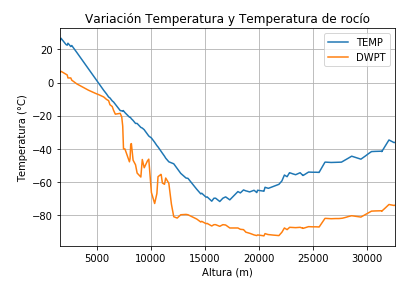
\includegraphics[width=\linewidth]{5thInstJun.png}
    \caption{22/Jun/2017}
	\end{subfigure}
    \caption{Variación de la temperatura y temperatura de rocío}
\end{figure}

\newpage

Enseguida se graficó la velocidad de los vientos en unidades de nudo.
\begin{figure}[h!]
	\begin{subfigure}[b]{0.5\linewidth}
    \raggedleft
	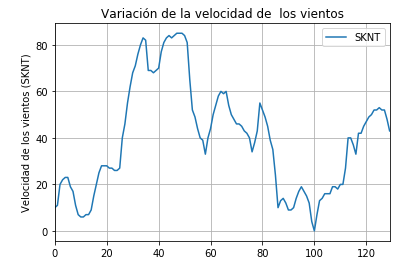
\includegraphics[width=\linewidth]{6thInstDec.png}
    \caption{22/Dic/2017}
	\end{subfigure}
	\begin{subfigure}[b]{0.5\linewidth}
    \raggedright
	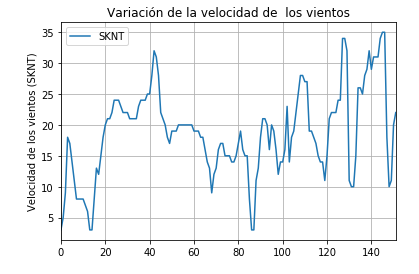
\includegraphics[width=\linewidth]{6thInstJun.png}
    \caption{22/Jun/2017}
	\end{subfigure}
    \caption{Variación de la velocidad del viento}
\end{figure}

Y por último se graficaron las variacion de la humedad relativa con cada medición.
\begin{figure}[h!]
	\begin{subfigure}[b]{0.5\linewidth}
    \raggedleft
	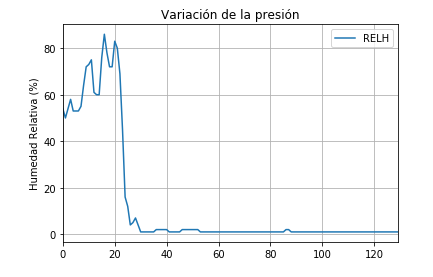
\includegraphics[height=0.15\textheight, width=\linewidth]{7thInstDec.png}
    \caption{22/Dic/2017}
	\end{subfigure}
	\begin{subfigure}[b]{0.5\linewidth}
    \raggedright
	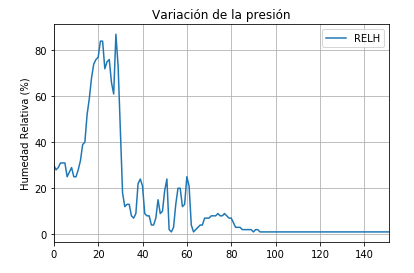
\includegraphics[height=0.15\textheight, width=\linewidth]{7thInstJun.png}
    \caption{22/Jun/2017}
	\end{subfigure}
    \caption{Variación de la humedad relativa}
\end{figure}

\section{Resultados}

En la Figura 1 se mostró la variación de la presión respecto a la altura en las cuales se observa un comportamiento exponencial decreciente: Conforme el globo metereológico asciende la presión desciende de acuerdo a la fórmula barométrica. Este cambio en la presión es independiente de los factores dados por las temporadas terrestres.

Después, en la Figura 2 se muestra el cambio de la temperatura respecto a la altura, donde se puede observar que en diciembre a partir de la tropopausa la temperatura no aumenta ni disminuye conforme incrementa la altitud. Sin embargo, en la gráfica de junio se nota que a partir de la tropopausa la temperatura incrementa con respecto a la altura.

Luego, en la Figura 3 se muestra el cambio de la temperatura y la temperatura de rocío en función de la altura, donde se puede notar que en junio las nubes son más propensas a formarse a mayor altitud que en diciembre. Debido a que la estación en la que se tomaron las mediciones es una zona árida en Nuevo México la formación de nubes no es tanta en las gráficas como se observaría en otras areas.

En la Figura 4 se muestra la variación de la velocidad del viento en el cual se puede notar que la velocidad del viento en junio es un poco más uniforme que en diciembre.

En la Figura 5 se muestra la humedad relativa en la que se puede apreciar que esta es mayor en la epoca de junio, que, de hecho, es más alta a la altura en la que es mas propenso formarse nubes como observamos en la Figura 3.

\section{Conclusión}

En conclusión, el análisis de datos y graficación no se puede realizar sin antes preparar bien a los datos que queremos estudiar para que sean leídos por el programa.

\newpage

\section{Bibliografía}
\begin{itemize}
\item Egbert Boeker and Rienk van Grondelle (2000). Environmental Physics (2nd ed.). Wiley.
\item Clive D. Rodgers (2000). Inverse Methods for Atmospheric Sounding: Theory and Practice. World Scientific.
\item A quick derivation relating altitude to air pressure Archived 2011-09-28 at the Wayback Machine. by Portland State Aerospace Society, 2004, accessed 05032011
\end{itemize}

\newpage

\title{Apéndice}

\begin{enumerate}
\item ¿Cuál es tu opinión general de esta actividad? ~\\~\\
Creo que me tarde mucho para nada, y no necesite usar funciones elegantes para cortar datos innecesarios como les paso a mis compañeros debido a que copie solamente lo que necesitaba del sitio de descarga

\item ¿Qué fue lo que más te agradó? ¿Lo que menos te agradó?~\\~\\
Lo que más me agrado fue la creación e interpretación de las gráficas y lo que menos me agrado solamente fue el prepararme para realizar la práctica

\item ¿Que consideras que aprendiste en esta actividad?  ~\\~\\
Aprendí que por más que paresca que pandas hace todo solito, a veces leer los datos no lo hace automaticamente

\item ¿Qué le faltó? ¿O le sobró?   ~\\~\\
Creo que le faltó un poco mas de enseñanza hacia el manejo de datos, debido a que se nos dificultó al principio y algunos aún no sabían como proceder cuando su programa leía objetos.

\item ¿Que mejoras sugieres a la actividad? ~\\~\\
únicamente que se explique mejor los problemas que hay al leer archivos y presentar algunas soluciones explícitas

\end{enumerate}

\end{document}
